% Бүлэг 3

\chapter{Системийн зохиомж} % Зарим нэг зөвлөмж
\label{Chapter3} % Энэ бүлэг рүү ишлэл хийх бол \ref{Chapter2} командыг ашигла 

\section{Үйл ажиллагааны диаграм}
\begin{figure}[htbp]
	\centering
	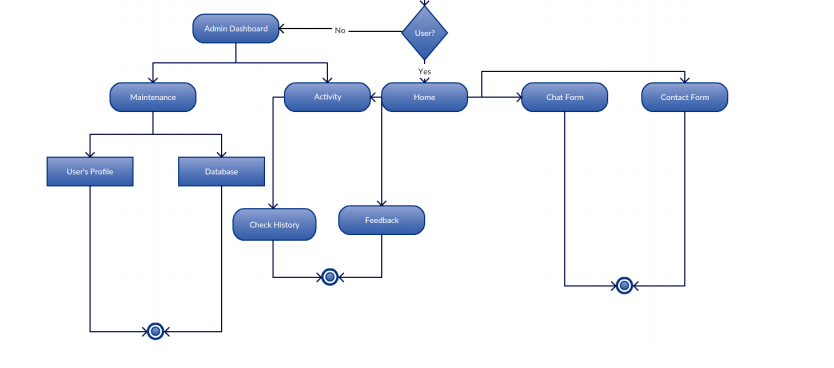
\includegraphics[scale=0.5]{Diagrams/Activity1}
	\caption[Үйл ажиллагааны диаграм]{Засвар, удирдлага}
	\label{fit:Interface}
\end{figure}
\begin{figure}[htbp]
	\centering
	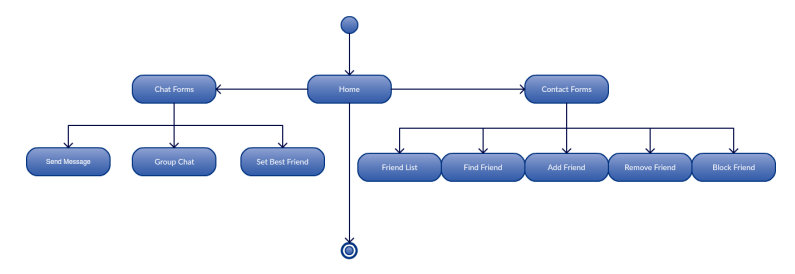
\includegraphics[scale=0.5]{Diagrams/Activity2}
	\caption[Үйл ажиллагааны диаграм]{Холбогдох, чат хэлбэр}
	\label{fit:Activity}
\end{figure}

\section{Класс диаграм}
\begin{figure}[htbp]
	\centering
	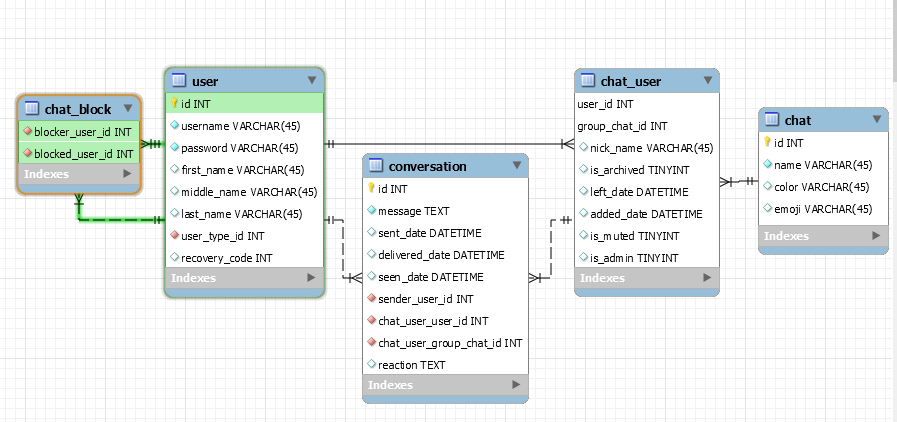
\includegraphics[scale=0.4]{Diagrams/ClassEntity}
	\caption[Класс диаграм]{Объектын холбоосын диаграм}
	\label{fit:Interface}
\end{figure}

\section{Дарааллын диаграм }

\section{Төлөвийн диаграм }

\section{Хэрэглэгчийн интерфейс }
\begin{figure}[htbp]
	\centering
	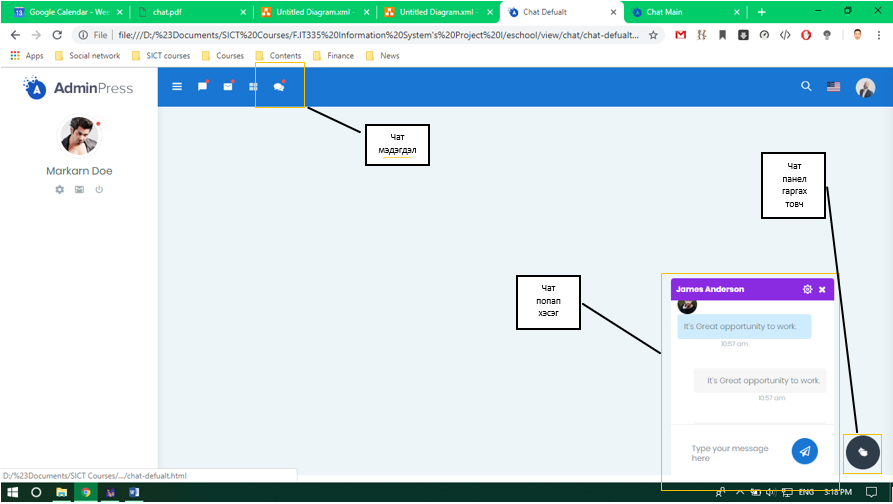
\includegraphics[scale=0.7]{Chart/Interface1}
	\caption[Хэрэглэгчийн интерфейс]{Чат мэдэгдэл, попап, панел товч}
	\label{fit:Interface}
\end{figure}
\begin{figure}[htbp]
	\centering
	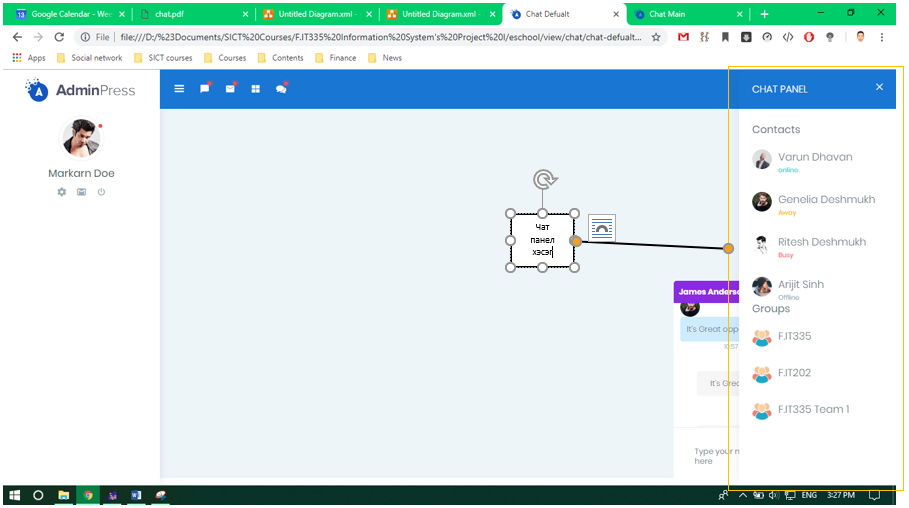
\includegraphics[scale=0.7]{Chart/Interface2}
	\caption[Хэрэглэгчийн интерфейс]{Чат панел хэсэг}
	\label{fit:Interface}
\end{figure}
\begin{figure}[htbp]
	\centering
	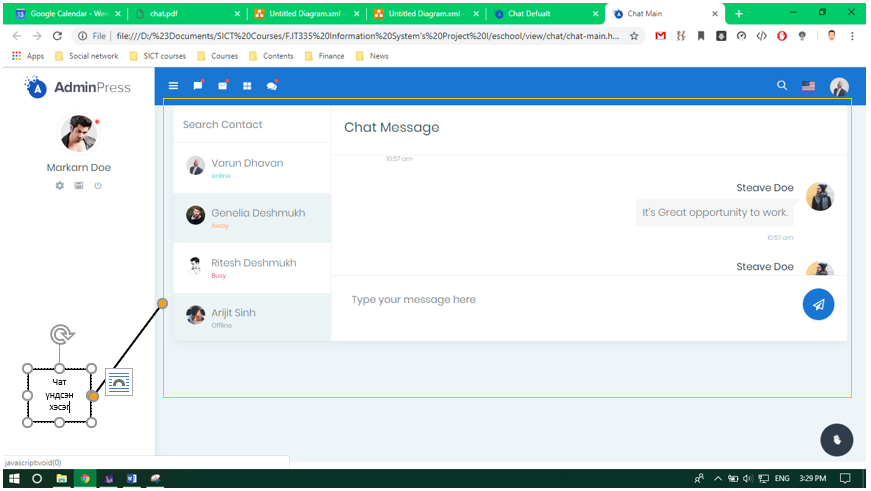
\includegraphics[scale=0.7]{Chart/Interface3}
	\caption[Хэрэглэгчийн интерфейс]{Чат үндсэн хэсэг}
	\label{fit:Interface}
\end{figure}
	
\section{Тестийн зохиомж}
	
